\documentclass[doc,a4paper]{apa7}
\usepackage[utf8]{inputenc}
\usepackage[T1]{fontenc}
\usepackage[style=apa, backend=biber, url=true]{biblatex}
\usepackage{booktabs}
\usepackage{graphicx}
\usepackage[export]{adjustbox}
\usepackage{listings,multicol}
\lstset{
  numbers=left,
  firstnumber=1,
  numberfirstline=true
}
\usepackage{varioref}
\usepackage{hyperref}
\usepackage{cleveref} % MUST be loaded in this exact order!
\usepackage{placeins}
\usepackage{tablefootnote}
\usepackage{xcolor}
\usepackage{array}
\usepackage{calc} % for calculating minipage widths
\usepackage{etoolbox}
\setlength{\emergencystretch}{3em} % prevent overfull lines
\providecommand{\tightlist}{%
  \setlength{\itemsep}{0pt}\setlength{\parskip}{0pt}}
\setcounter{secnumdepth}{-\maxdimen} % remove section numbering
\usepackage{bookmark}
\IfFileExists{xurl.sty}{\usepackage{xurl}}{} % add URL line breaks if available
\urlstyle{same}
\hypersetup{
  colorlinks=true,
  linkcolor={blue},
  filecolor={Maroon},
  citecolor={blue},
  urlcolor={blue},
  pdfcreator={Christophe Pallier <christophe@pallier.org>}}

\setlength{\headheight}{23pt}
\addtolength{\topmargin}{-9pt}
\renewcommand{\topfraction}{.9}
\renewcommand{\floatpagefraction}{.9}

% --------------------------- Content -----------------------------------------------------------------

\title{Goxpyriment: A Go Framework for Behavioral and Cognitive Experiments}
\shorttitle{Let's go experiment!}

\authorsnames{Christophe Pallier, Julie Bonnaire, Marie-France Fourcade}
\authorsaffiliations{Cognitive Neuroimaging Unit, CNRS INSERM CEA}

\authornote{\addORCIDlink{Christophe Pallier}{0000-0002-3324-666X} Correspondence should be addressed to  C. Pallier, Cognitive Neuroimaging Unit, Neurospin, Gif-sur-Yvette, F-91191, France. E-mail: christophe@pallier.org. I would like to thank Luca Bonatti and Raphael Bordas for alpha testing this software. The authors have no conflicts of interest to disclose.}

\keywords{framework, library, stimulus presentation, timing, behavioral experiments, psychophysics, psychology}

\addbibresource{biblio.bib}

\abstract{We introduce \texttt{goxpyriment}, an open-source software
  framework for programming behavioral and cognitive experiments in
  the Go programming language. It addresses two recurrent practical
  difficulties of existing Python-based tools: the runtime-environment
  complexity that complicates deployment across laboratories, and the
  unpredictable pauses that automatic memory management can introduce
  during timing-critical sections. Because Go is a compiled language
  that can natively embed assets (e.g., graphics, audio files, and
  stimulus lists), \texttt{goxpyriment} compiles an entire experiment
  into a single, self-contained executable with no runtime
  dependencies, so that distributing an experiment amounts to copying
  one file. Users can just click on the executable within their file
  browser and do not need to open a terminal and use the command line
  (but they can if they want/need to).  The programming interface is
  inspired by Expyriment \parencite{krause2014}. It provides an array
  of visual stimuli (text, shapes, images, Gabor patches, motion
  clouds, \ldots) and audio capabilities (WAV playback and tone
  generation). For precise timing, response times are obtained by
  using operating-system event timestamps recorded at
  hardware-interrupt time rather than by continuous polling, and the
  garbage collector can be suspended for the duration of a trial. We
  characterize the resulting timing behaviour with the hardware-based
  protocol of the timing mega-study \parencite{bridges2020}, reporting
  visual, auditory, and trigger latencies across several hardware
  configurations. The framework ships with over forty example
  experiments that serve as reusable templates for common
  paradigms. \texttt{goxpyriment} is released under the Apache License
  2.0 and is freely available at
  \url{https://github.com/chrplr/goxpyriment}.}

\begin{document}
\maketitle


\section{Introduction}\label{introduction}

Experiment-control software provides the foundation for empirical
behavioral and cognitive neuroscience: the temporal precision of
stimulus delivery and response recording, the ergonomics of experiment
programming, and the ease of deploying experiments to laboratory
hardware each affect the quality and reproducibility of empirical
data. Over the past two decades, Python has become the dominant
language for experiment programming, primarily through libraries such
as PyEPL \parencite{pyepl_2007}, VisionEgg \parencite{visionegg_2008},
Expyriment \parencite{krause2014} and PsychoPy
\parencite{peirce2019}. Before that, MATLAB with the Psychophysics
Toolbox \parencite{brainard1997, kleiner2007} was the de facto
standard in many laboratories and is still in use in some of
them. More recently, web-based frameworks such as jsPsych
\parencite{deleeuw2015, deleeuw2023} and lab.js
\parencite{henninger2022} have enabled large-scale online data
collection.

Each class of tool involves tradeoffs. MATLAB, extended with the
Psychtoolbox, is convenient to generate visual or auditory stimuli and
offers good timing on well-configured hardware. Yet Psychtoolbox
scripts written on Windows most often do not work out of the box on
Linux (and vice-versa). MATLAB can also be costly for institutions
that cannot obtain academic licenses (as is the case for some
non-degree-granting research institutions).  Python tools provide a
more open programming environment with a large scientific ecosystem.
Python-based experiments can also achieve high-precision timing, for
example by relying on the psychtoolbox Python module which provides
pieces of the Psychtoolbox-3 (see
\url{https://pypi.org/project/psychtoolbox/}). However, the use of
Python introduces practical difficulties. For instance, deploying an
experiment to a computer that does not already have a compatible
Python environment requires package management (pip, venv, conda, uv,
\ldots) and can be a source of breakage across operating-system
versions. For example, installing the \texttt{psychopy} module under
Linux fails while compiling the wxPython package when no precompiled
wheel is available. Second, Python's garbage collector can introduce
unpredictable pause times that corrupt the timing of
stimulus presentation and response recording during the critical trial
loop. Web-based tools have an obvious advantage in terms of facility
of deployment, but browser-mediated stimulus presentation is subject
to event-loop latency that makes precise timing difficult
\parencite{bridges2020, anwylirvine2021}.

The Go programming language \parencite{golang} offers a different set
of tradeoffs. Go is a deliberately small language with a limited
feature set and few alternative ways to express a given operation,
which tends to make programs easy to read and to reason about
\parencite{donovan2016}. It is statically typed, and its conventions
encourage explicit error checking, so that many mistakes surface at
compile time rather than at run time, which is a huge time saver for
the programmer.  Moreover, two properties of Go make it an
attractive language to program and distribute experiments.  First, Go
(cross-)compiles to native machine code and can produce self-contained
binaries that embed the stimuli and experiment lists and have thus no
runtime dependencies. Second, its garbage collector is concurrent and
can be suspended for the duration of a timing-critical section. These
properties motivated our choice of Go as the basis for a behavioral
experiment library that prioritizes deployment simplicity and timing
control.

The present article describes the design and capabilities of
\texttt{goxpyriment}, details its timing architecture, and
characterizes its temporal precision empirically. We highlight three
contributions: (1) zero-dependency deployment via single compiled
binaries that simplify distribution across laboratory hardware; (2) a
timing architecture that obtains response times from operating-system
event timestamps and that can suspend garbage collection during
trials, whose behaviour we quantify using the protocol of the timing
mega-study \parencite{bridges2020}; and (3) the existence of a gallery
of more than forty examples of experiments.

{\small
% float=tp (not *t): the doc class is one-column, so a starred full-width
% float has nothing to span and gets deferred to the end of the document.
\lstinputlisting[float=tp, label=paritycode, caption={Example of a Parity Decision experiment}, lineskip=-5pt, breaklines=true, breakatwhitespace=true, basicstyle=\small\ttfamily]{parity-decision.go}
\par}

\section{Framework Design}\label{framework-design}

\subsection{Foundation: SDL3}

\texttt{Goxpyriment} relies on the Simple DirectMedia Layer, a
cross-platform development library designed to provide low-level
access to audio, keyboard, mouse, joystick, and graphics hardware
\parencite{sdl3}.  SDL has been used to develop thousands of
commercial games as well as many emulators. Bindings for many
programming languages exist, notably for Python with the \verb|pygame|
library \parencite{pygame}. Because of its large user and developer
bases, SDL is actively maintained and keeps up with modern hardware.
Goxpyriment uses the latest version of this library, SDL3, through the
go-sdl3 bindings \parencite{gosdl3}.


\subsection{Single-Binary Deployment (Zero Dependencies)}\label{single-binary-deployment}

Go compiles programs into a single statically linked executable with
no external runtime dependencies. Crucially, the \texttt{go-sdl3}
package embeds the pre-built SDL3 runtime libraries \parencite{sdl3}
directly into the executable, so that no library needs to be installed
separately on the target machine.  In addition, the stimuli,
experimental lists, fonts, and other assets can be embedded in the
binary too. As a result, distributing an experiment requires copying
just one file; there is no need to manage virtual environments,
package versions, or interpreter installations across laboratory
computers. This substantially reduces the operational overhead of
installing experiments on multiple machines or sharing materials with
collaborators.

Another important consequence of the fact that the executable is
statically linked is that the user does not have to worry about
potential changes in future versions of the library which could impact
the behavior of their program. This promotes reproducibility.


\subsection{Programming interface: a simple example}\label{example}

Listing~\vref{paritycode} provides an example of a simple experiment
implementing a parity decision task where participants have to decide
if a number is even or odd.

\begin{itemize}
\item Line 12: An \texttt{Experiment} object that manages the
window, renderer, and audio subsystems must be created
early. Calling it also parses the command-line to get the subject's
code and whether the experiment should run in fullscreen mode or not.

\item Lines 16--36: This part of the code prepares the stimuli. Lines
31--36 are the most Go-specific: they create a map (a.k.a. associative
array or dictionary in other programming languages) associating each
number to a graphic texture. By pre-building these textures, we ensure
that they will be displayed as quickly as possible in the presentation
loop (we could have called \texttt{stimuli.NewTextLine()} in the loop,
saving a few lines at the cost of recomputing the texture at each
iteration).

\item Lines 41--56: This part of the code deals with the presentation
  loop. It is wrapped in a \texttt{Run} call that catches quitting
  events: if the participant presses the Escape key or closes the
  window, the library catches the resulting internal signal, safely
  flushes the data file to disk, and shuts down the SDL subsystems,
  ensuring that data is preserved even if a session is aborted
  prematurely. Line 47, the function \texttt{ShowAndGetRT()} presents
  the visual stimulus, waits for one of the given keys, then returns
  the reaction-time.
\end{itemize}

\subsection{Timestamps, Garbage Collection Control, ...}

Response timing in \texttt{goxpyriment} exploits SDL3 OS-level event
timestamps. The \verb|ShowAndGetRT| function used in the parity example is
a wrapper for:

\noindent%
\begin{lstlisting}[numbers=none,basicstyle=\small]
  onset,_ := exp.ShowTS(stim)
  key,eventTS,_ := exp.Keyboard.GetKeyEventTS(keys,
                                              timeoutMs)
  rt := int64(eventTS - onset) / 1_000_000
\end{lstlisting}

\texttt{ShowTS()} displays the stimulus \texttt{stim}, blocking until
the next screen flip when VSYNC is enabled, and returning a
time-stamp for that event (in ns).  When VSYNC is disabled,
\texttt{ShowTS()} returns immediately, supporting variable
refresh rate (VRR) monitors.

\verb|GetKeyEventTS()| scans the keyboard and returns the code of the
key pressed and a timestamp (in ns) for it. This timestamp is
populated by the OS input subsystem at hardware-interrupt time
(nanoseconds since SDL initialization).  Because SDL events carry
their timestamp (information that pygame discards), the event remains in
the queue with its original timestamp regardless of how much
computation occurs between stimulus onset and response collection.  By
comparing the response timestamp with the \texttt{ShowTS()} timestamp,
reaction times can be computed without interpreter overhead
(hardware-level lags at the keyboard or mouse can, of course, still be
present). An advantage of this approach is that there is no need to
poll the HID device continuously to detect events: a complex sequence
of stimuli can be programmed and every event remains available, with
its original timestamp, to be processed later when needed.

To reduce the likelihood of latencies, goxpyriment provides additional functions:

\begin{description}
\item[Explicit Garbage Collection Control] Go, like Python or
  JavaScript, has a memory garbage collector. This can introduce
  unpredictable pauses that corrupt timing. However, unlike Python or
  Javascript, Go allows the programmer to suspend the garbage
  collector.  This can be used in \texttt{goxpyriment}'s
  timing-critical loops to prevent garbage-collection during a trial.

\item[High-Precision Streams] For paradigms with dense, high-speed
  stimulus sequences (e.g., retinotopic stimulation),
  \texttt{goxpyriment} provides specialized stream functions such as
  \texttt{PresentStreamOfImages}. These functions disable garbage
  collection, drain the event queue, and busy-wait at the sub-frame
  level to ensure that each stimulus onset is scheduled accurately. A
  \texttt{TimingLog} records the target and actual onsets for post-hoc
  verification, as well as the timing of keys pressed during the
  presentation of the stream.

\item[Real-Time Scheduling Priority] On Linux, an experiment built with
  \texttt{goxpyriment} requests the \texttt{SCHED\_FIFO} real-time
  scheduling policy for itself at start-up (priority 50 by default),
  rather than relying on the user to remember a \texttt{chrt} prefix on
  the command line --- which is in any case impossible when the program
  is launched by clicking its icon. The request is made with
  \texttt{sched\_setscheduler()} on the main thread, to which the Go
  runtime has been pinned, so that the elevation applies to the thread
  that runs the trial loop. Under the default (\texttt{SCHED\_OTHER})
  policy the kernel may deschedule the process at any point, including
  between a stimulus onset and the trigger that marks it; this is the
  dominant source of the rare, large latencies that otherwise survive
  the measures above.

  The request is not silently mandatory. It requires a system-level
  grant (an \texttt{rtprio} limit for the user, set in
  \texttt{/etc/security/limits.d/}), and if that grant is absent the
  program reports the reason and continues at normal priority rather
  than refusing to run. It can be disabled with the
  \texttt{-no-realtime} flag --- useful when debugging, since a
  breakpoint hit on a real-time thread can leave the desktop
  unresponsive --- and the priority can be changed with
  \texttt{-realtime-priority}. The policy actually obtained is recorded
  in the session's system report, so that a data set carries evidence of
  the conditions under which it was collected rather than of the
  conditions that were intended.
\end{description}

\subsection{Triggers}

To communicate with external recording equipment, such as fMRI, EEG,
and MEG systems, \verb|Goxpyriment| provides generic functions for
reading from and writing to parallel and serial ports. Moreover, the
current version implements TTL input/output interfaces for specific
USB-serial devices: the DLP-IO-8 (see
\url{https://github.com/chrplr/dlp-io8-g}) and an Arduino Mega 2560
utilizing a custom protocol (see
\url{https://github.com/chrplr/neurospin-meg-ttl-box}), and for an
Ethernet-based device: the LabJack T4
(\url{https://labjack.com/products/labjack-t4}). Adding support for
new hardware is facilitated by the availability of the source code for
the current devices.

A notable feature of the Go language is that it makes asynchronous
function execution trivial by simply prepending the \verb|go| keyword
to a function call. For example, \verb|go pp.Pulse(5, 200)| sends a
200~ms TTL pulse to line 5 of the parallel port in a 'fire-and-forget'
manner. The function runs as a concurrent process and control returns
immediately to the caller, allowing the program to proceed without
delay—for example, to continue with stimulus presentation.


\subsection{Miscellaneous additional features}

This parity decision example only demonstrates a tiny part of the features
provided by the framework.

For example, it is possible to build the experiment around a
hierarchical structure of blocks and trials, over which the program
can iterate, following a pattern inspired by Expyriment
\parencite{krause2014}. Each trial is a collection of factors that can
be randomized and logged. Data collection is handled by an
\texttt{exp.Data} object, which writes to a CSV file with metadata
headers providing extensive information about the computer OS and
hardware, timestamps, etc.

Another thing which is not transparent from the source code is the fact
that \texttt{goxpyriment} provides a graphical
\texttt{GetParticipantInfo} dialog that opens (optionally) before the
main experiment window (see Fig.~\ref{fig:getinfo}). This allows the
experimenter to input subject IDs, select experimental conditions from
discrete menus, and toggle settings like fullscreen mode. These values
are automatically recorded in the output data file header.

\begin{figure}[t]
\centering
\begin{tabular}{l}
  \textbf{A.}\\
  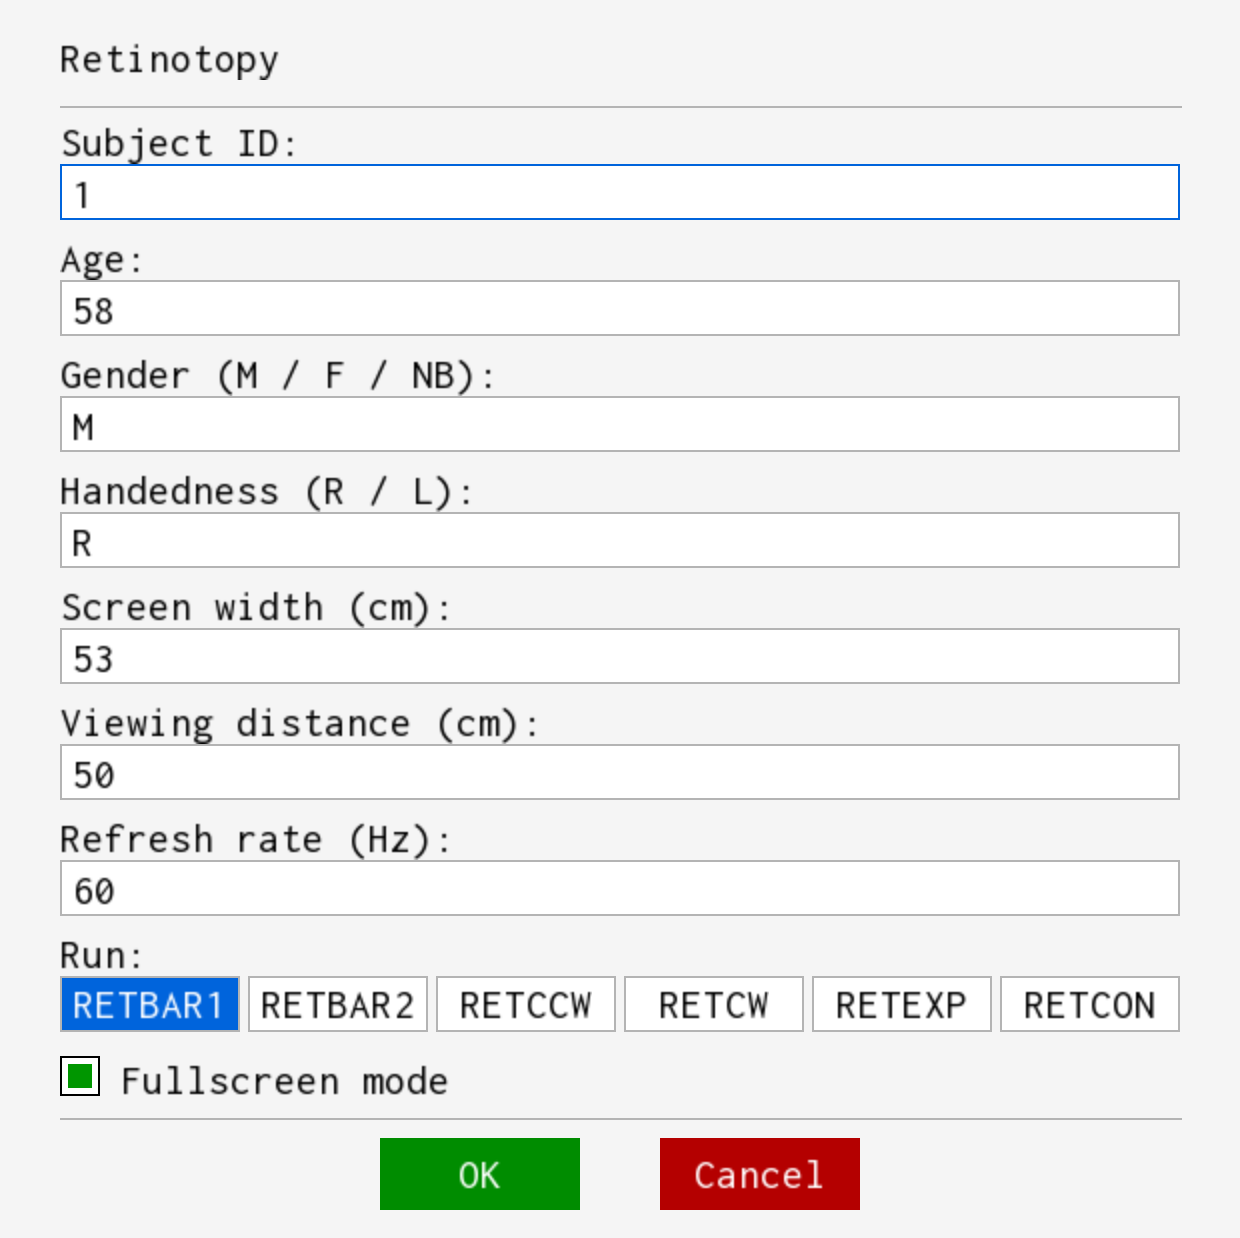
\includegraphics[width=0.5\textwidth,valign=t]{UI1.png} \\[.5cm]
  \textbf{B.}\\
  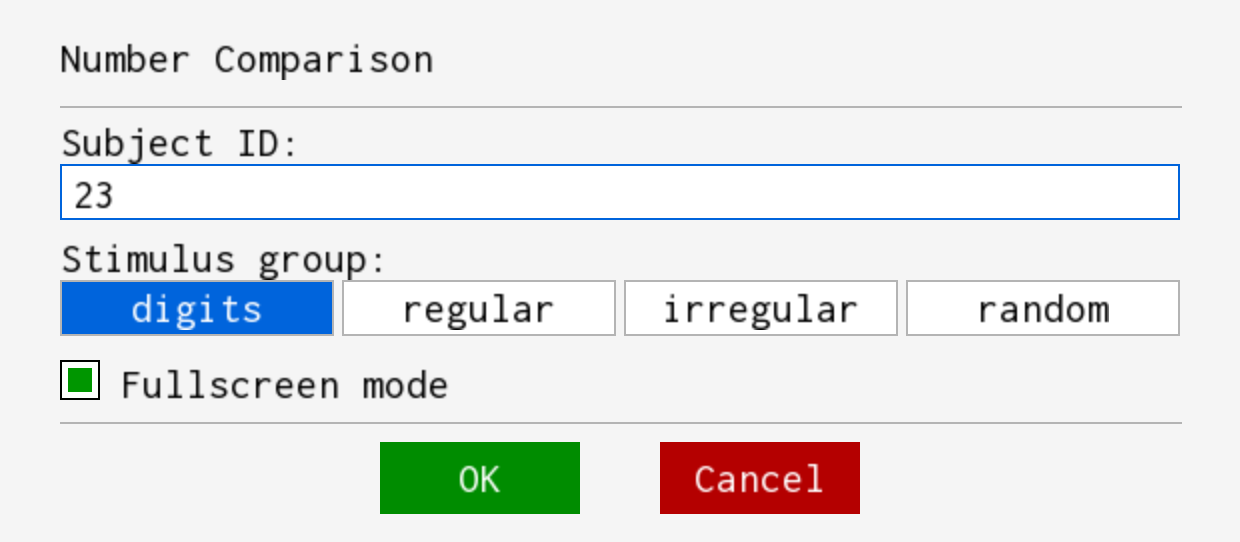
\includegraphics[width=0.5\textwidth,valign=t]{UI2.png} \\
\end{tabular}
\caption{Examples of \texttt{GetParticipantInfo} dialogs for
  \emph{Retinotopy} (A.) and \emph{Number-Comparison} (B.), two paradigms
  provided in the examples accompanying the library. These UIs makes it
  practical for the experimenter to choose among a small set of
  options without typing, which reduces setup errors when launching an
  experiment from a desktop shortcut or file manager. Note that which
  fields appear in the UI is configurable. It is also possible to
  pass the information as arguments on the command-line and skip these
  UIs.}
\label{fig:getinfo}
\end{figure}


% Every number in this section was measured on 2026-08-16/17 and is traceable
% to a capture file. Where a measurement is missing it says so rather than
% reusing an older figure taken under different conditions.
\section{Timing Validation}\label{timing-verification}

To characterise temporal precision we adopt the hardware-measurement protocol of
the timing mega-study \parencite{bridges2020}, which compared a range of
lab-based and online experiment generators using a Black Box Toolkit (BBTK).
External instruments record the physical events---light onsets from a photodiode
on the screen, sound onsets, and TTL edges on a digital line---independently of
the computer under test, so the reported latencies do not depend on the timing of
the machine being measured.

We depart from that protocol in one respect, and the departure turned out to
matter. Alongside the BBTK we recorded the same events with a Digilent Analog
Discovery~3 (AD3) sampling two analogue channels at 100~kS/s on a single
timebase. The BBTK quantises event onsets to 0.25~ms and applies a detection
threshold whose value is not reported in its output; the AD3 records the
waveform, so the onset criterion is a choice made at analysis time and stated
with the result. Two independent instruments measuring the same events by
different routes is also the only way we found to discover what each was adding:
several of the results below correct earlier measurements of ours that were
instrument artefacts rather than properties of the apparatus.

\subsection{What is measured, and why the three are not interchangeable}

We report three quantities that are routinely conflated under the word
``timing'':

\begin{description}
\item[Accuracy] the mean lag between an event and its physical
  consequence---trigger to light, light to sound. Accuracy is a constant offset,
  and a constant offset can be compensated by scheduling the stimulus earlier.
\item[Precision] the trial-to-trial scatter of that lag. It cannot be
  compensated, and it is what propagates into a single-trial reaction time.
\item[Stability] whether the lag holds over a block. A lag that slides has an
  ordinary standard deviation and an ordinary mean, and every within-channel
  statistic looks correct while it happens; only a comparison against an
  external clock reveals it.
\end{description}

Stability is the one most often omitted, and it is the one that fails silently.

\subsection{The framework's own timestamps track the display}

A stimulus generator reports an onset time, and an experiment's reaction times
are measured from it. If that reported time advances on a clock other than the
display's, the error grows for as long as the block lasts. This is not
hypothetical: an earlier version of \texttt{goxpyriment} held each frame to a
schedule derived from the nominal refresh rate, and on a Radeon Pro W5700 the
reported onsets walked away from the photons at $-4.73$~ppm---2.3~ms per
eight-minute block, exceeding a frame within the hour---while the program's own
frame-interval statistics remained immaculate.

The mechanism is worth stating because it generalises beyond this framework. On
that machine the GPU and the CPU keep independent crystals; its loop cadence
differs from the nominal rate by $-4.20$~ppm. While onsets were timestamped with
a schedule advancing on the CPU clock and the panel ran on the GPU clock, that
crystal difference \emph{was} the drift. The two figures are the same quantity.

The current version anchors each onset on the instant
\texttt{SDL\_RenderPresent} returns wherever the driver blocks on the retrace,
which re-establishes the phase from hardware on every frame. Measured against a
photodiode over 1000 cycles ($\approx$8.3~min) per run:

\begin{center}
\begin{tabular}{lrr}
\hline \hline
Machine & before & after \\
\hline
Raspberry Pi 4 (V3D, kmsdrm)      & 14~ms / 8~min & $+0.01$~ppm (0.006~ms) \\
Radeon Pro W5700 (radeonsi, X11)  & $-4.73$~ppm   & $+0.13$~ppm (0.066~ms) \\
\hline
\end{tabular}
\end{center}

The W5700 row is the stronger evidence: there the failure was measured, its
magnitude was predicted from the crystal offset, and it is now measured gone,
while the machine's cadence is still $-4.20$~ppm from nominal. That the cadence
and the drift now disagree by a factor of 32 is what demonstrates the onsets are
following the panel rather than the schedule.

\subsection{Configuration dominates the hardware}

Table~\ref{timings} reports the two machines. The pattern across it is that
differences between \emph{configurations} of one machine exceed differences
between machines.

\begin{table*}[tb]
\caption{Timing measured with a photodiode on the screen and, for the audio
  rows, the machine's line output; 100~kS/s, both channels on one acquisition,
  onsets at a 10\% criterion. Both machines drove the same Dell 1905FP panel at
  1280$\times$1024, 60.0197~Hz, with the photodiode in the same position. Cycle:
  12 frames on, 18 off. The criterion is named because it matters: this panel's
  10--90\% transition takes 16.3~ms, a full frame, so where the onset is declared
  on that ramp shifts every lag below by up to 16~ms. It costs nothing in
  precision --- the trial-to-trial scatter is 8--23~$\mu$s at every level --- and
  sets everything in accuracy, which is why a latency quoted without its
  criterion is not reproducible even on the same rig.}
\label{timings}
\scriptsize
\begin{tabular}{llrrrl}
\hline \hline
Machine & Configuration & $n$ & Mean & SD & Quantity \\
\hline
\multicolumn{6}{l}{\emph{Trigger to light}} \\
Pi 4    & GPIO, kmsdrm            & 300 & 23.43~ms & 0.075~ms & TTL edge $\rightarrow$ 10\% light \\
W5700   & DLP-IO8 (USB), X11      & 481 & 54.88~ms & 0.296~ms & \\
W5700   & DLP-IO8 (USB), kmsdrm   & 286 & 22.55~ms & 0.057~ms & \\
\\
\multicolumn{6}{l}{\emph{Light to sound (audio-visual synchrony), 1024-frame buffer}} \\
Pi 4    & on-board codec, PipeWire & 481 & 49.88~ms & 6.17~ms & 10\% light $\rightarrow$ tone envelope \\
W5700   & Scarlett Solo, PipeWire  & 646 & 23.34~ms & 6.54~ms & \\
\\
\multicolumn{6}{l}{\emph{Flip timestamp to photons (stability)}} \\
Pi 4    & kmsdrm  & 1000 & $+0.01$~ppm & 0.128~ms & slope; de-trended SD \\
W5700   & X11     & 1000 & $+0.13$~ppm & 0.278~ms & \\
\\
\multicolumn{6}{l}{\emph{Presentation}} \\
Pi 4    & kmsdrm  & 481 & 197.840~ms & 0.070~ms & 12-frame duration, 50\% criterion \\
Pi 4    & kmsdrm  & 480 & 499.820~ms & 0.012~ms & cycle period \\
\hline
\end{tabular}
\end{table*}

\paragraph{The display stack costs two frames.} On the W5700, stopping the X
server and running the same binary on bare KMS/DRM---same machine, panel,
photodiode position and trigger device---moved the trigger-to-light lag from
54.88~ms to 22.55~ms and the scatter from 0.296~ms to 0.057~ms. The 32.4~ms is
almost exactly two frames, consistent with an X11 Present path plus a driver
swapchain queueing ahead of scanout; under KMS/DRM the application page-flips
directly to the CRTC. The panel is not implicated: its 10--90\% transition
measures 16.29~ms on the Pi and 17.28~ms here, with the same shape.

None of this is visible from inside the program. Both configurations report that
the driver blocks, sub-ppm stability against the panel, and frame intervals
with sub-millisecond scatter. An experiment reporting an absolute onset would be
32~ms wrong under X11 with no internal evidence of it.

\paragraph{The trigger device is not the bottleneck it is assumed to be.} A
USB-serial trigger (DLP-IO8) under KMS/DRM gives 0.057~ms of scatter---better
than a directly-driven GPIO line on the Pi (0.075~ms). We had initially
attributed the W5700's wider spread to its USB link; the KMS/DRM run shows the
display server was responsible.

\paragraph{Audio jitter is the buffer, and it is deterministic.} Recording the
line output electrically, the audio onset scatters by one buffer period divided
by $\sqrt{12}$:

\begin{center}
\begin{tabular}{lrrrr}
\hline \hline
Buffer (frames at 48~kHz) & period & measured SD & $\mathrm{period}/\sqrt{12}$ & torn tones \\
\hline
\phantom{0}256 & \phantom{0}5.33~ms & \phantom{0}2.36~ms & \phantom{0}1.54~ms & 100 / 483 \\
\phantom{0}512 & 10.67~ms & \phantom{0}3.34~ms & \phantom{0}3.08~ms & 10 / 500 \\
1024           & 21.33~ms & \phantom{0}6.17~ms & \phantom{0}6.16~ms & 0 / 481 \\
2048           & 42.67~ms & 12.27~ms & 12.32~ms & 0 / \phantom{0}60 \\
\hline
\end{tabular}
\end{center}

Prediction and measurement agree to within 8\% at every point, and the same
relation held on a USB audio interface on the other machine. The scatter is not
noise: the tone's position within the buffer grid advances by
$(\mathrm{cycle} \bmod \mathrm{period})$ each trial and wraps, a deterministic
beat. On the Pi, with a 499.830~ms cycle and a 10.667~ms buffer, this predicts
$+1.503$~ms per trial with a $-9.163$~ms wrap; the measured values were
$+1.500$ and $-9.170$~ms. A cycle chosen as a whole multiple of the buffer
period removes the beat entirely.

Below 1024 frames the audio tears: 2.0\% of tones at 512 and 20.7\% at 256
contained audible silences. At 512 the audio server responded to repeated
underruns by adding a buffer period mid-run, stepping the latency by
$+10.85$~ms and relocating the very quantity being measured. This is a floor set
by the hardware, not by the server: with the server stopped and the device
opened directly through ALSA, every one of 463 tones was torn.

Throughout all of this the software-side statistic---the interval between the
visual flip and the moment the tone was handed to the audio device---read
$0.080 \pm 0.035$~ms. The framework does its part correctly; everything above
happens downstream of it, and no host-side number reveals any of it.

\subsection{Recommendations}

\begin{itemize}
\item Measure the configuration, not the machine. The largest effects we found
  (32~ms from the display server, 79~ms and 4$\times$ the jitter from the audio
  buffer) are settings, not hardware.
\item If absolute onset latency matters---EEG, MEG, cross-modal work---run
  without a display server, and measure rather than assume.
\item Choose the audio buffer by measurement: as small as the machine sustains
  without tearing, since both latency and jitter scale with it.
\item State the onset criterion with any latency, and the buffer size with any
  audio figure.
\item Report stability, not only mean and SD. A drifting lag is invisible to
  both.
\end{itemize}

The suite that produces these measurements ships with the framework
(\texttt{tests/Timing-Tests/}) and writes the configuration---display mode,
audio device and buffer, scheduling policy, onset source, and the pacing branch
each frame took---into every data file, so that a capture carries the conditions
it was collected under.

% TODO(revision): still to add —
%   (a) same-hardware comparison against PsychoPy, per bridges2020's protocol;
%   (b) GC-on versus GC-suspended frame-interval distributions (the harness
%       already runs the pair; the analysis is not written);
%   (c) recovered response-time accuracy with the BBTK generating programmed
%       responses at known delays;
%   (d) the Dell Precision 5490 configuration, for a third display stack
%       (Wayland), which is the one where SDL_RenderPresent does not block.


\section{Gallery of Examples}

The repository provides over forty demos and examples of classic
psychology paradigms, including the Stroop task, Attentional Blink
(RSVP), Masked Priming, Retinotopic mapping for fMRI, and adaptive
threshold estimation using the QUEST algorithm. These examples serve
as both functional templates and a gallery of the framework's
capabilities.


TODO: expand this section, insert a more structured description of Gallery of examples (and mention demos).

The examples and demos are available as pre-compiled binaries in the
Releases tab of the github repository.  Yet, compiling all of them
locally can be achieve in three steps: 1) install Go on your
machine; 2) clone or download goxpyriment repository 3) run the
`build.all` shell script.



\section{Comparison with Existing Tools}\label{comparison-with-existing-tools}

Table~\ref{tab:comparison} summarizes key properties of \texttt{goxpyriment}
alongside five other experiment frameworks.

\begin{table*}[tb]
\caption{Comparison of selected experiment frameworks.}
\label{tab:comparison}
\footnotesize
\begin{tabular}{@{}
  >{\raggedright\arraybackslash}p{0.17\textwidth}
  >{\raggedright\arraybackslash}p{0.14\textwidth}
  >{\raggedright\arraybackslash}p{0.14\textwidth}
  >{\raggedright\arraybackslash}p{0.14\textwidth}
  >{\raggedright\arraybackslash}p{0.14\textwidth}
  >{\raggedright\arraybackslash}p{0.14\textwidth}@{}}
\toprule
Property & goxpyriment & Expyriment & PsychoPy & PTB (MATLAB) & jsPsych \\
\midrule
Language        & Go           & Python        & Python            & MATLAB           & JavaScript \\
Deployment      & Single binary & pip/conda    & Standalone or pip & MATLAB license   & CDN / npm \\
GC control      & Explicit disable & No        & No                & N/A              & No \\
VSYNC sync      & Yes (SDL3)   & Yes (SDL2)    & Yes (Pyglet/PTB)  & Yes              & No \\
Hardware triggers & Yes        & Yes           & Yes               & Yes              & No \\
Response device API & Unified  & Device-specific & Device-specific & Device-specific & N/A \\
Event timestamp & SDL3 hardware & pygame timer & iohub/PTB clock  & \texttt{GetSecs} ($\mu$s) & Browser clock \\
Stimulus set    & Moderate     & Moderate      & Extensive         & Extensive        & Moderate \\
GUI builder     & No           & No            & Yes (Builder)     & No               & No \\
Online deployment & No         & No            & Partial (PsychoJS) & No              & Yes \\
Reference       & This paper   & \cite{krause2014} & \cite{peirce2019} & \cite{brainard1997} & \cite{deleeuw2023} \\
\bottomrule
\end{tabular}
\end{table*}

\texttt{goxpyriment} resembles Expyriment in its API design: a central
experiment object, a \texttt{present()}-based stimulus API, a
structured trial-loop model, and output to \texttt{.csv}-format files
with metadata. The code for a simple experiment (Parity Decision) is
provided in Listing~\ref{paritycode}. The primary technical differences
are the use of Go rather than Python and the use of SDL3 rather than
the older Pygame/SDL2 stack. From the user's point of view,
\texttt{goxpyriment} adds \emph{stream} objects which, as their name
indicates, allow displaying sequences of stimuli with tightly
controlled timing.

Table~\ref{tab:comparison} necessarily simplifies; each framework has
strengths that a compact matrix cannot convey. PsychoPy, in
particular, offers a graphical Builder interface, a larger and
extensively documented stimulus set, mature online deployment through
PsychoJS, and a large user community. The Psychtoolbox remains a
reference for low-level timing control on well-configured
hardware. Relative to these established tools, \texttt{goxpyriment} is
very young: it has no graphical builder, no online deployment, and a
more limited stimulus library. Its distinctive contributions are
therefore deployment simplicity and an explicit timing architecture
rather than breadth of features. The entries in
Table~\ref{tab:comparison} describe design characteristics; measured
timing comparisons on identical hardware are reported in
Section~\ref{timing-verification}.


\subsection{Expandability}

The availability of the source code makes it easy to expand
goxpyriment, e.g., adding support for new hardware. Given a clear
specification for an hardware interface, an human, or an AI coding
assistant can quickly generate Go code for this hardware taking
example from the existing packages.


\section{Limitations and Future Directions}\label{limitations-and-future-directions}

\textbf{No Eye-tracker support.} There is none for the moment. This is a
target for future releases. The coding effort is expected to be small
as some code has already been written to interact through TCP/IP to
control some of the trigger devices.

\textbf{No video recording}. While there is currently some support for
recording audio responses and measuring naming times, the framework
does not currently allow to capture videos (unless one controls a
videorecorder through the serial interface).  As SDL3 supports recording
video, this feature might be implemented in the future.

\textbf{No way of sending results to a web server}.  Currently,
results files are saved locally. In some situations, it could be
useful to send the (anonymized) results to an on-line database, for
example using a REST api.

\textbf{Online deployment.} Currently, \texttt{goxpyriment} does not
support web-based deployment. As Go can compile to web assembly (wasm)
and SDL3 supports EMSCRIPTEN (\url{https://emscripten.org/}), it is an
achievable goal. We actually have a proof of concept, having
successfully implemented several examples of the gallery to run in the
browser. However, work remains to be done to support all goxpyriment
functions in the browser.  When this is achieved, the exact same
source code will support web and local deployment.

\textbf{Language barrier.}  Researchers who are unfamiliar with Go,
that is, the vast majority, will need to invest a bit of time in
getting acquainted with the language.  To this end, many web resources
exist, for example, \url{https://go.dev/tour/} and
\url{https://gobyexample.com/}. As Go is a descendant of C, the syntax
will be familiar to people who know a language of the same family,
e.g., Java or Javascript. Finally, the examples and the migration
guide we provide at \url{https://chrplr.github.io/goxpyriment}, are
also meant to ease the transition. AI-Coding tools can help a lot in
porting existing matlab or python code, adapting existing experiments,
or creating new ones.

\textbf{Name of the project.} The name ``goxpyriment'' is quite hard to
pronounce, it is recommanded to call the framework  'gox-py'.

\clearpage

\section{Declarations}

\subsection{Funding}

No funding was received to assist with this project nor with the preparation of this manuscript.

\subsection{Conflict of interest/Competing interest}

The authors have no competing interests to declare that are relevant to the content of this article.

\subsection{Ethics approval}

Not applicable.

\subsection{Consent to participate}

Not applicable.

\subsection{Consent for publication}

Not applicable.

\subsection{Availability of data and materials}

\subsection{Code availability}

The source code of \texttt{goxpyriment} is available under the Apache
License 2.0 at
\url{https://github.com/chrplr/goxpyriment}. All example experiments
described in this article are included in the repository. No empirical
data are reported in this article.

\subsection{Authors Contributions}\label{author-contributions}

\textbf{Christophe Pallier}: Conceptualization, Software
implementation, Documentation and Paper Writing, with assistance from
\textbf{Claude Sonnet 4.6} and \textbf{Gemini 2.5}. Consistent with
current editorial norms \parencite{natureportfolio2023,
  springernature2023}, Claude and Gemini are listed under Author
Contributions rather than as a named author, because authorship
requires the capacity to take accountability for the work.  Christophe
Pallier takes full responsibility for all content. \textbf{Julie
  Bonnaire} and \textbf{Marie-France Fourcade} set up the timing
measurement system and performed tests.

\clearpage

\printbibliography

\end{document}
